\documentclass[12pt, a4paper, oneside]{ctexart}
\usepackage{amsmath, amsthm, amssymb, bm, color, framed, graphicx, mathrsfs}
\usepackage{listings}
\usepackage{xcolor}      %代码着色宏包
\usepackage{geometry}
\usepackage[hidelinks]{hyperref} %隐藏链接
\geometry{margin=1in}
\lstset{
    basicstyle= \scriptsize\tt,
    %行号
    numbers=left,
    rulesepcolor=\color{red!20!green!20!blue!20},
    escapeinside=``,
    xleftmargin=2em,xrightmargin=2em, aboveskip=1em,
    %背景框
    framexleftmargin=0mm,
    frame=shadowbox,
    %背景色
    % backgroundcolor=\color[RGB]{245,245,244},
    %样式
    keywordstyle=\color{blue}\bfseries,
    identifierstyle=\bf,
    numberstyle=\color[RGB]{0,192,192},
    commentstyle=\it\color[RGB]{96,96,96},
    stringstyle=\rmfamily\slshape\color[RGB]{128,0,0},
    %显示空格
    showstringspaces=false,
    breaklines,
    columns=flexible,
}
\lstdefinestyle{Python}{
    language        = Python,
    basicstyle      = \ttfamily,
    keywordstyle    = \color{blue},
    keywordstyle    = [2] \color{teal}, % just to check that it works
    stringstyle     = \color{green},
    commentstyle    = \color{red}\ttfamily
}

\title{\textbf{工程实践与科技创新IV-J}\\课程作业}
\author{pangbo}
\date{\today}
\linespread{1.5}
\definecolor{shadecolor}{RGB}{241, 241, 255}
\newcounter{problemname}
\newenvironment{problem}{\begin{shaded}\stepcounter{problemname}\par\noindent\textbf{题目\arabic{problemname}. }}{\end{shaded}\par}
\newenvironment{solution}{\par\noindent\textbf{解答. }}{\par}
\newenvironment{note}{\par\noindent\textbf{题目\arabic{problemname}的注记. }}{\par}

\begin{document}

\maketitle

\begin{problem}
    MLQP反向传播算法推导。
\end{problem}

    为方便表述,现将推导过程中的符号及其含义简述如下:

    \begin{itemize}
        \item $x_i^{(k)}(n)$代指第$n$次迭代时,第$k$层输入向量的第$i$个元素。
        \item $t_j^{(k)}(n)$代指第$n$次迭代时,第$k$层第$j$个神经元激活函数输入值。
        \item $u_{ji}^{(k)}(n)$、$v_{ji}^{(k)}(n)$代指第$n$次迭代时,连接第$k-1$层第$i$个神经元与第$k$层第$j$个神经元的权重值,$u$、$v$分别代指二次项与一次项的系数。
        \item $y_j^{(k)}(n)$代指第$n$次迭代时,第$k$层第$j$个神经元的输出, $y_j^{(k)}(n) = x_j^{(k+1)}(n)$。
        \item $d_j(n)$代指第$n$次迭代时,输出层第$j$个神经元应当输出的值。
        \item $e_j(n)$代指第$n$次迭代时,输出层第$j$个神经元输出与实际值的差,即$e_j(n)=d_j(n)-y_j(n)$。
        \item $\varepsilon(n)$代指第$n$次迭代输出的均方误差。
    \end{itemize}

    首先考虑输出层参数关于损失函数的梯度,

    \begin{align*}
        \frac{\partial \varepsilon}{\partial u_{ji}^{(k)}} &= \frac{\partial \varepsilon}{\partial e_j}\frac{\partial e_j}{\partial y_j} \frac{\partial y_j}{\partial t_j} \frac{\partial t_j}{\partial u_{ji}^{(k)}}\\
        &= e_j\cdot (-1) \sigma'(t_j){x_i^{(k)}}^2\\
        &= -e_j\sigma'(t_j){x_i^{(k)}}^2
    \end{align*}

    \begin{align*}
        \frac{\partial \varepsilon}{\partial v_{ji}^{(k)}} &= \frac{\partial \varepsilon}{\partial e_j}\frac{\partial e_j}{\partial y_j} \frac{\partial y_j}{\partial t_j} \frac{\partial t_j}{\partial v_{ji}^{(k)}}\\
        &= e_j\cdot (-1) \sigma'(t_j)x_i^{(k)}\\
        &= -e_j\sigma'(t_j)x_i^{(k)}
    \end{align*}

    \begin{align*}
        \frac{\partial \varepsilon}{\partial b_j^{(k)}} &= \frac{\partial \varepsilon}{\partial e_j}\frac{\partial e_j}{\partial y_j} \frac{\partial y_j}{\partial t_j} \frac{\partial t_j}{\partial b^{(k)}}\\
        &= e_j\cdot (-1) \sigma'(t_j)\cdot 1\\
        &= -e_j\sigma'(t_j)
    \end{align*}

    为方便表述,记$\delta^{(k)}_j=-e_j\sigma'\left(t_j^{(k)}\right)$,于是$\frac{\partial \varepsilon}{\partial u_{ji}^{(k)}}=\delta^{(k)}_j{x_i^{(k)}}^2$、$\frac{\partial \varepsilon}{\partial v_{ji}^{(k)}}=\delta^{(k)}_j{x_i^{(k)}}$、$\frac{\partial \varepsilon}{\partial b_{ji}^{(k)}}=\delta^{(k)}_j$。

    对于隐藏层神经元,首先分析每个神经元输出对于最终损失的贡献值,即损失函数对于$y_{j}^{(k-1)}$的导数。

    \begin{align*}
        \frac{\partial \varepsilon}{\partial y_{j}^{(k-1)}} &=-\sum_{p} e_{p}\sigma'(t_{p}^{(k)}) \frac{\partial t_p^{(k)}}{ \partial y_{j}^{(k-1)}}\\
        &=-\sum_{p} e_{p}\sigma'(t_{p}^{(k)}) \frac{\partial t_p^{(k)}}{ \partial x_{j}^{(k)}}\\
        &=-\sum_{p} e_{p}\sigma'\left(t_{p}^{(k)}\right)\left(2u^{(k)}_{pj}x_{j}^{(k)}+v^{(k)}_{pj}\right)\\
        &=\sum_{p} \delta_p^{(k)}\left(2u^{(k)}_{pj}x_{j}^{(k)}+v^{(k)}_{pj}\right)
        % &=-\sum_{k} \delta_{k}(n) w_{k j}(n)
    \end{align*}

    基于此我们可以给出隐藏层每个参数对损失函数的导数。
    
    \begin{align*}
        \frac{\partial \varepsilon}{\partial u_{ji}^{(k-1)}} &= \frac{\partial \varepsilon}{\partial y_{j}^{(k-1)}} \frac{\partial y_j^{(k-1)}}{\partial t_j^{(k-1)}} \frac{\partial t_j^{(k-1)}}{\partial u_{ji}^{(k-1)}}\\
        &= \frac{\partial \varepsilon}{\partial y_{j}^{(k-1)}} \sigma'\left(t_j^{(k-1)}\right){x_i^{(k-1)}}^2
    \end{align*}
    \begin{align*}
        \frac{\partial \varepsilon}{\partial v_{ji}^{(k-1)}} &= \frac{\partial \varepsilon}{\partial y_{j}^{(k-1)}} \frac{\partial y_j^{(k-1)}}{\partial t_j^{(k-1)}} \frac{\partial t_j^{(k-1)}}{\partial v_{ji}^{(k-1)}}\\
        &= \frac{\partial \varepsilon}{\partial y_{j}^{(k-1)}} \sigma'\left(t_j^{(k-1)}\right){x_i^{(k-1)}}
    \end{align*}
    \begin{align*}
        \frac{\partial \varepsilon}{\partial b_{ji}^{(k-1)}} &= \frac{\partial \varepsilon}{\partial y_{j}^{(k-1)}} \frac{\partial y_j^{(k-1)}}{\partial t_j^{(k-1)}} \frac{\partial t_j^{(k-1)}}{\partial b_{ji}^{(k-1)}}\\
        &= \frac{\partial \varepsilon}{\partial y_{j}^{(k-1)}} \sigma'\left(t_j^{(k-1)}\right)
    \end{align*}

    用带$\delta^{(k)}_j$的式子表示各层参数的梯度。
    
    \begin{align*}
        \frac{\partial \varepsilon}{\partial u_{ji}^{(k)}} &= \delta^{(k)}_j {x^{(k)}_i}^2 = \delta^{(k)}_j {y^{(k-1)}_i}^2\\
        \frac{\partial \varepsilon}{\partial v_{ji}^{(k)}} &= \delta^{(k)}_j {x^{(k)}_i} = \delta^{(k)}_j {y^{(k-1)}_i}^2\\
        \frac{\partial \varepsilon}{\partial b_{j}^{(k)}} &= \delta^{(k)}_j
    \end{align*}
    其中,$\delta^{(k)}_j$值如下。
    $$
        \delta^{(k)}_j = \frac{\partial \varepsilon}{\partial t_{j}^{(k)}}=\begin{cases}
            -e_j\sigma'\left(t_j^{(k)}\right)\text{,第k层为输出层}\\
            \sigma'\left(t_j^{(k)}\right)\sum_{p} \delta_p^{(k+1)}\left(2u^{(k+1)}_{pj}x_{j}^{(k+1)}+v^{(k+1)}_{pj}\right)\text{,第k层为隐藏层}
        \end{cases}
    $$
\begin{problem}
    使用编程语言为MLQP模型实现反向传播算法,训练一个带一个隐藏层的MLQP模型,并比较三个不同学习率下的训练效率与决策边界。
\end{problem}

    代码实现基于上述推导结果进行,模型与参数更新的核心代码位于文件\verb|MLQP.py|、\verb|optimizer.py|内。这部分代码包括3个主要部分。
    \begin{itemize}
        \item 前向传播
    \begin{lstlisting}[language=Python]
for layer_id in range(1,self.layers_nr):
    self.Tk[layer_id] = np.matmul(self.Uk[layer_id],np.square(self.Yk[layer_id-1])) + np.matmul(self.Vk[layer_id],self.Yk[layer_id-1]) + self.Bk[layer_id]
    self.Yk[layer_id] = self.sigmoid(self.Tk[layer_id])
    \end{lstlisting}
    \item 反向传播
    \begin{lstlisting}[language=Python]
# MSE损失函数
# self.DeltaK[-1] = (self.Yk[-1] - self.tag) * self.Yk[-1] * (np.ones_like(self.Yk[-1])-self.Yk[-1])

# 交叉熵损失函数
self.DeltaK[-1] = self.Yk[-1] - self.tag

for layer_id in range(self.layers_nr-2,0,-1):
    self.DeltaK[layer_id] = np.matmul((self.Uk[layer_id+1].T*self.Yk[layer_id]*2+self.Vk[layer_id+1].T),self.DeltaK[layer_id+1]) \
        * self.Yk[layer_id] \
        * (np.ones_like(self.Yk[layer_id])-self.Yk[layer_id])
    \end{lstlisting}
    \item 参数更新(SGD)
    \begin{lstlisting}[language=Python]
model = self.model
for layer_id in range(1,model.layers_nr):
    self.detUk[layer_id] = np.square(model.Yk[layer_id-1]).T * model.DeltaK[layer_id]
    self.detVk[layer_id] = model.Yk[layer_id-1].T * model.DeltaK[layer_id]
    self.detBk[layer_id] = model.DeltaK[layer_id]
    model.Uk[layer_id] -= lr*self.detUk[layer_id]
    model.Vk[layer_id] -= lr*self.detVk[layer_id]
    model.Bk[layer_id] -= lr*self.detBk[layer_id]
    \end{lstlisting}
    \item 参数更新(SGDM)
    \begin{lstlisting}[language=Python]
model = self.model
for layer_id in range(1,model.layers_nr):
    self.detUk[layer_id] = lr2*model.DeltaK[layer_id] * np.square(model.Yk[layer_id-1].T) + momentum*self.detUk[layer_id]
    self.detVk[layer_id] = lr*model.DeltaK[layer_id] * model.Yk[layer_id-1].T + momentum*self.detVk[layer_id]
    self.detBk[layer_id] = lr*model.DeltaK[layer_id] + momentum*self.detBk[layer_id]
    model.Uk[layer_id] -= self.detUk[layer_id]
    model.Vk[layer_id] -= self.detVk[layer_id]
    model.Bk[layer_id] -= self.detBk[layer_id]
    \end{lstlisting}
    \end{itemize}
    
    我首先研究了不同学习率对模型训练的影响,我分别使用0.1/0.01/0.001的学习率训练1000轮模型。模型的决策分界面如图\ref{Fig-MLQP-lr-compare-boundary}所示,图中蓝色与红色点代表测试数据集中两类数据点。模型训练过程中的损失函数与准确率如图\ref{Fig-MLQP-lr-compare-logging}所示,从上到下分别为学习率0.1/0.01/0.001的曲线,每个子图的纵坐标尺度不相同;图中黑色折线代表损失函数值,红色折线代表模型对训练数据集预测的准确率,蓝色折线代表模型对测试数据集预测的准确率。
    \begin{figure}[htbp]
        \centering
        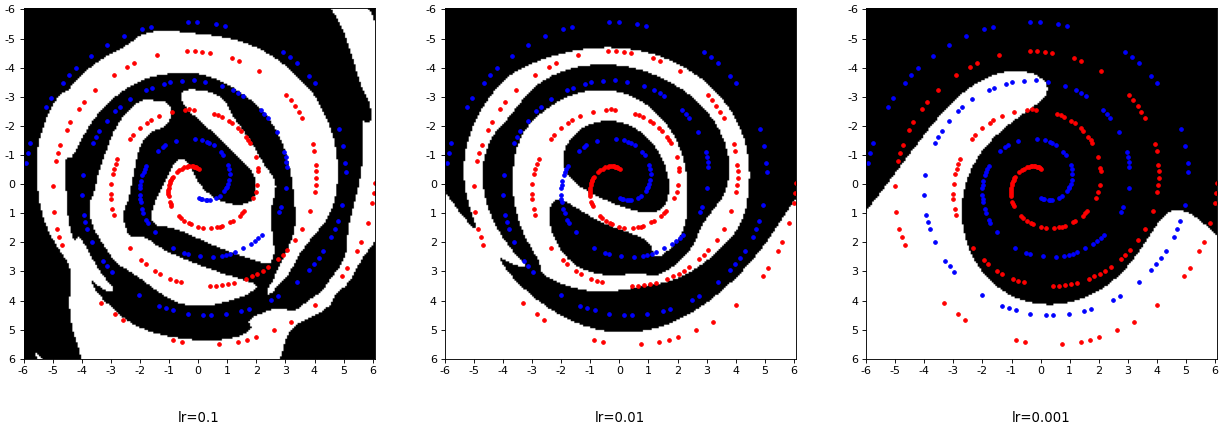
\includegraphics[width=0.9\textwidth]{figures/lr_compare_boundary.png}
        \caption{MLQP模型不同学习率下1000轮训练后决策边界图}
        \label{Fig-MLQP-lr-compare-boundary}
    \end{figure}
    
    \begin{figure}[htbp]
        \centering
        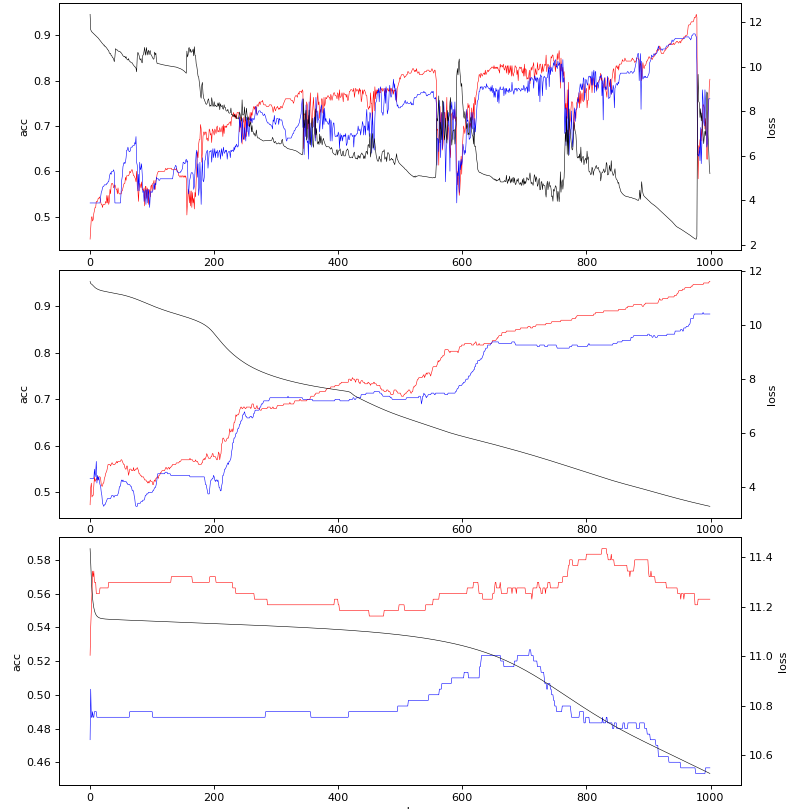
\includegraphics[width=1.0\textwidth]{figures/lr_compare_logging.png}
        \caption{MLQP模型不同学习率下训练过程中损失函数值与准确率曲线}
        \label{Fig-MLQP-lr-compare-logging}
    \end{figure}

    从图\ref{Fig-MLQP-lr-compare-logging}中可以看出,较高的学习率(如0.1)可以加快参数更新速率,但也可能导致参数更新过快产生波动;较小的学习率(如0.01)可以减小参数更新速率,但参数更新过慢,达到同样训练效果需要的时间更长,也更可能被困于局部最优点。

    我选择使用动态调整学习率的方法更新模型参数,首先用较大的学习率快速更新参数,如果训练过程中连续200轮没有有效提升,则将学习率降低为十分之一。类似于模拟退火算法,这样的动态学习率既可以加快前期训练速度,也可以避免后期模型参数跳变。




    经过2000轮训练,单一MLQP模型的决策边界图如图\ref{Fig-MLQP-boundary}所示,模型正确分类出了测试数据集中全部300个点。

    \begin{figure}[htbp]
        \centering
        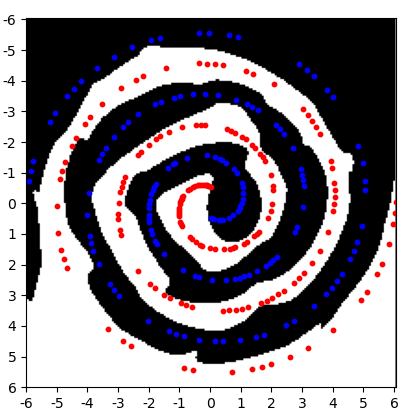
\includegraphics[width=0.5\textwidth]{figures/MLQP_boundary.png}
        \caption{MLQP模型2000轮训练后决策边界图}
        \label{Fig-MLQP-boundary}
    \end{figure}

    训练过程中模型的损失函数值与准确率变化曲线如图\ref{Fig-MLQP-logging}所示,图中黑色折线代表损失函数值,红色折线代表模型对训练数据集预测的准确率,蓝色折线代表模型对测试数据集预测的准确率。

    \begin{figure}[htbp]
        \centering
        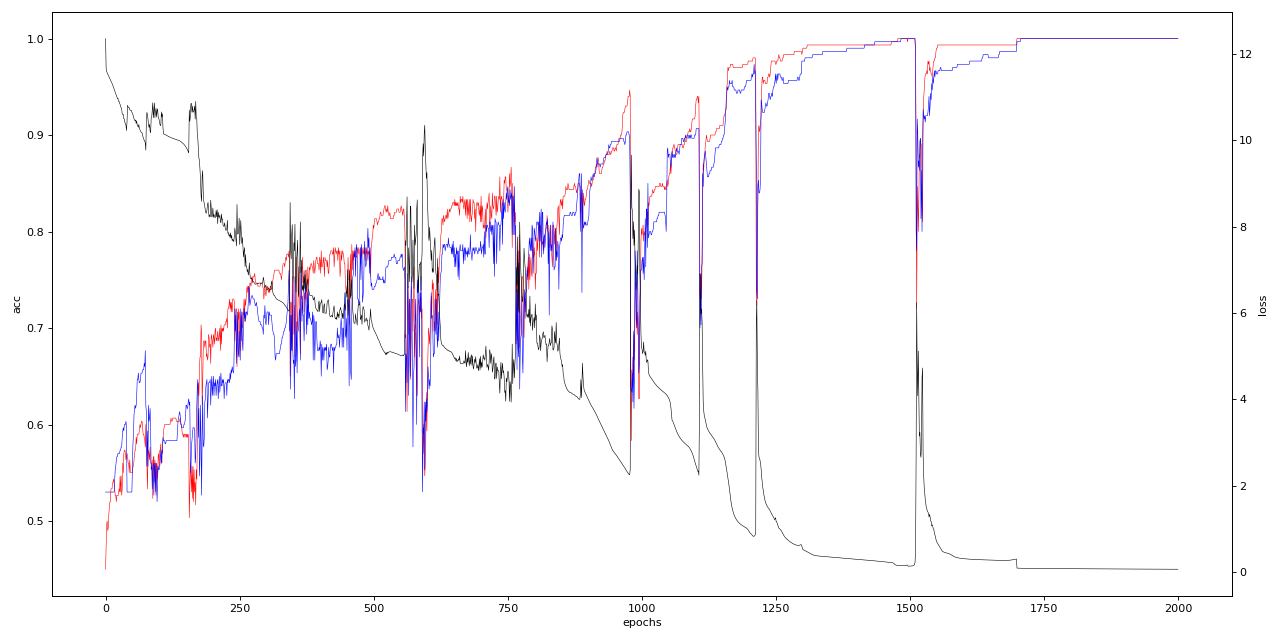
\includegraphics[width=1.0\textwidth]{figures/MLQP_logging.png}
        \caption{MLQP模型训练过程中损失函数值与准确率曲线}
        \label{Fig-MLQP-logging}
    \end{figure}

    我也保存了训练过程中的模型,并分别绘制出其决策边界,如图\ref{Fig-MLQP-process-boundary}所示。

    \begin{figure}[htbp]
        \centering
        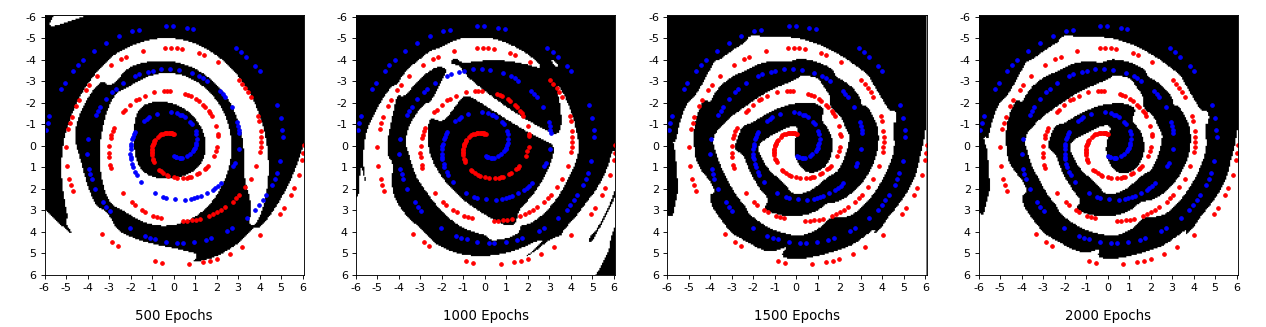
\includegraphics[width=1.0\textwidth]{figures/MLQP_process_boundary.png}
        \caption{MLQP模型训练过程中的决策边界变化}
        \label{Fig-MLQP-process-boundary}
    \end{figure}

    训练过程中,模型的ROC曲线如图\ref{Fig-MLQP-CrossEntropy-ROC}所示,模型的AUC大约在1250轮时达到1.0。

    \begin{figure}[htbp]
        \centering
        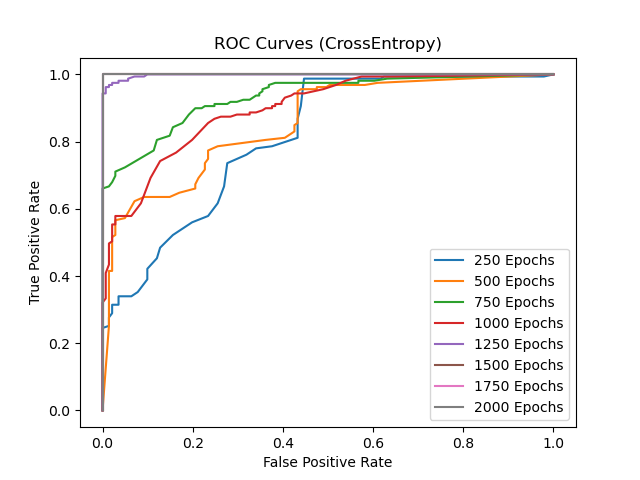
\includegraphics[width=0.6\textwidth]{figures/CrossEntropy_ROC.png}
        \caption{训练过程中模型的ROC曲线(交叉熵)}
        \label{Fig-MLQP-CrossEntropy-ROC}
    \end{figure}

    由于均方差(MSE)损失函数与sigmoid函数的组合会导致模型输出值在0、1附近时梯度趋于0,因此MSE函数并不是分类模型的理想损失函数。基于此,上述的模型训练过程中我使用了交叉熵(CrossEntropy)损失函数,该损失函数表达式为
    $$L=\frac{1}{N}\sum_{i}L_i=\frac{1}{N}\sum_{i}-[y_i\cdot log(p_i)+(1-y_i)\cdot log(1-p_i)]$$
    交叉熵函数与sigmoid函数组合可以获得较为理想的梯度,有助于提高模型参数更新效率。

    作为对比,我也使用了MSE函数在其他条件相同的情况下训练了相同的模型,训练过程中模型的ROC曲线如图\ref{Fig-MLQP-MSE-ROC}所示,相比使用交叉熵训练的曲线图\ref{Fig-MLQP-CrossEntropy-ROC},MSE的训练效率明显低于交叉熵,且模型的AUC最终未在2000轮训练时达到1.0。

    \begin{figure}[htbp]
        \centering
        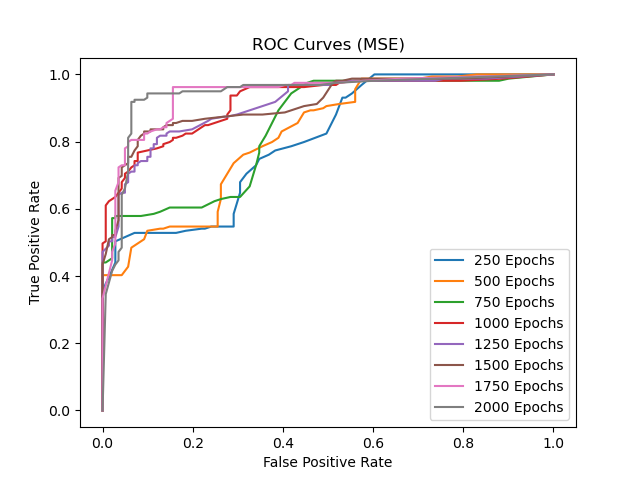
\includegraphics[width=0.6\textwidth]{figures/MSE_ROC.png}
        \caption{训练过程中模型的ROC曲线(均方差)}
        \label{Fig-MLQP-MSE-ROC}
    \end{figure}

    除此之外,我使用了Xavier初始化、引入了动量(Momentum)提高训练效率。

\begin{problem}
    分别使用先验知识和随机将分类问题拆分为4或9个子问题,并对每个子问题分别训练MLQP模型并构造min-max模型,比较不同模型的训练效率与决策边界。
\end{problem}
    
    我首先将两类数据点分别以X轴为界将数据点各自分为两类,然后两两组合组成四组训练数据,分别放入四个模型进行训练,然后使用min-max方法组合四个模型。

    先验拆分模型的决策边界如图\ref{Fig-minmax-axis-boundary}所示,每个子模型的决策边界如图\ref{Fig-minmax-axis-each-boundary}所示,子模型训练过程的损失函数、准确率变化如图\ref{Fig-minmax-axis-logging}所示。
    
    从整体结果来看,先验拆分的min-max模型在大约1000轮训练后已经可以分辨出绝大多数数据点,且决策边界相当平滑,不足之处在于模型对X轴(即数据集拆分边缘)附近的数据点的分类结果不够精确。
    
    从图\ref{Fig-minmax-axis-each-boundary}中可以看出,第2、3子模型只是简单上下分类,因此大部分分类工作是由1、4模型完成的。

    从图\ref{Fig-minmax-axis-logging}中可以看出1、4子模型训练速度明显慢于2、3子模型。整体而言,在400轮训练时已经可以得到较为理想的结果。

    \begin{figure}[htbp]
        \centering
        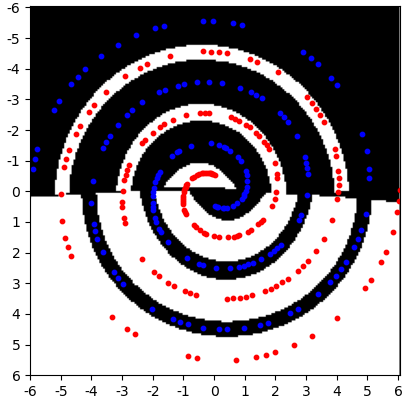
\includegraphics[width=0.6\textwidth]{figures/minmax_axis_boundary.png}
        \caption{先验拆分min-max模型决策边界}
        \label{Fig-minmax-axis-boundary}
    \end{figure}

    \begin{figure}[htbp]
        \centering
        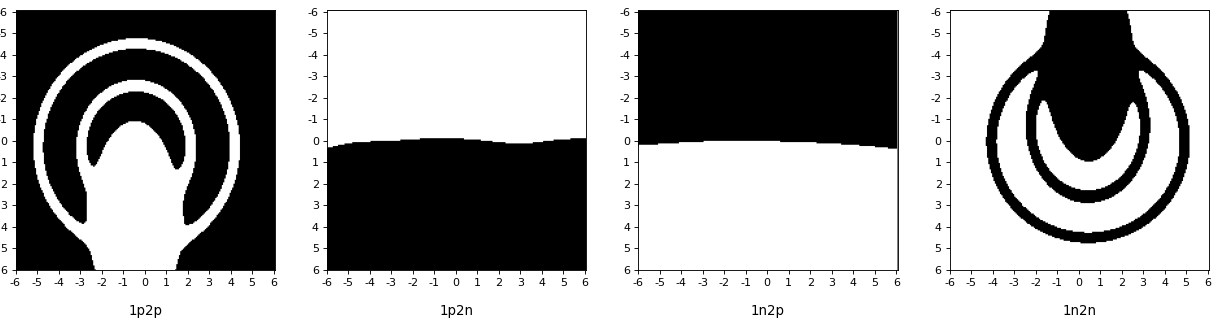
\includegraphics[width=1.0\textwidth]{figures/minmax_axis_each_boundary.png}
        \caption{先验拆分min-max每个子模型的决策边界}
        \label{Fig-minmax-axis-each-boundary}
    \end{figure}

    \begin{figure}[htbp]
        \centering
        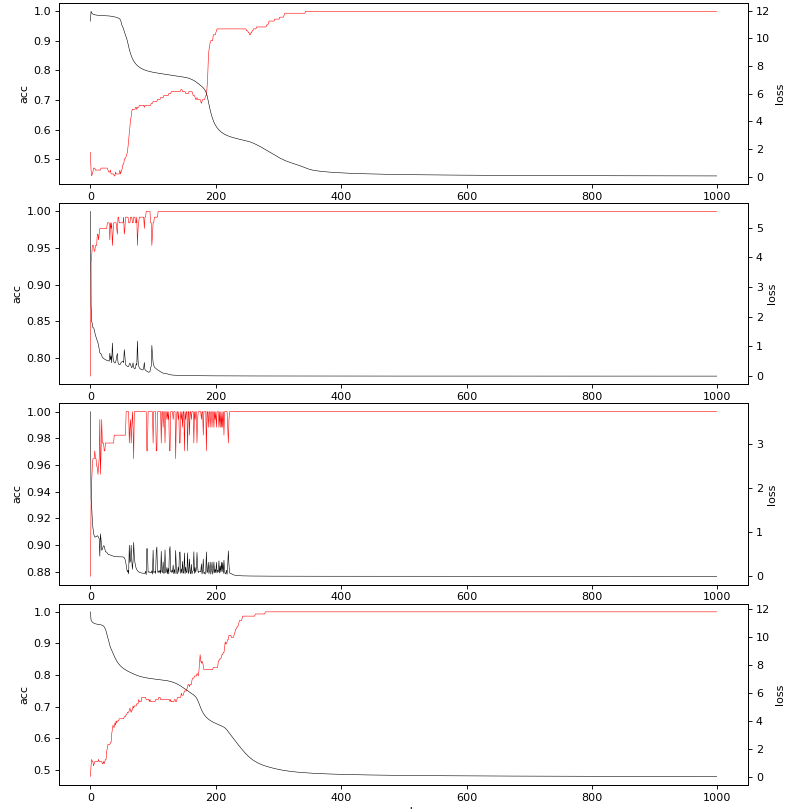
\includegraphics[width=1\textwidth]{figures/minmax_axis_logging.png}
        \caption{先验拆分min-max每个子模型的损失函数、准确率变化}
        \label{Fig-minmax-axis-logging}
    \end{figure}

    此后,我又按照随机顺序拆分训练集,并尽可能保证训练数据集的平衡,分别训练四个模型。与我最初的预期不同,随机拆分训练2000轮之后的结果仍略差于先验拆分1000轮训练后的结果,在测试训练集上的准确率大约为93\%。

    对于随机拆分数据集的min-max模型,决策边界如图\ref{Fig-minmax-random-boundary}所示,每个子模型的决策边界如图\ref{Fig-minmax-random-each-boundary}所示,子模型训练过程的损失函数、准确率变化如图\ref{Fig-minmax-random-logging}所示。

    从图\ref{Fig-minmax-random-each-boundary}中可以看出,随机拆分训练集中每个子图均具有一定程度的特征,但所有子图组合而成的决策边界图(图\ref{Fig-minmax-random-boundary})并不能足够完整地复现整体数据集特征。

    根据实验结果,我得出结论,在当前问题下,使用先验知识将数据集按照坐标轴拆分可以在更短的训练时间内获得更好的训练结果。

    \begin{figure}[htbp]
        \centering
        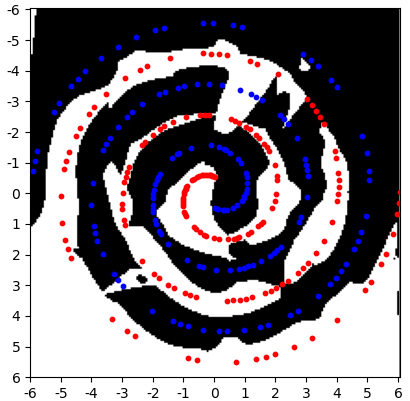
\includegraphics[width=0.6\textwidth]{figures/minmax_random_boundary.png}
        \caption{随机拆分min-max模型决策边界}
        \label{Fig-minmax-random-boundary}
    \end{figure}

    \begin{figure}[htbp]
        \centering
        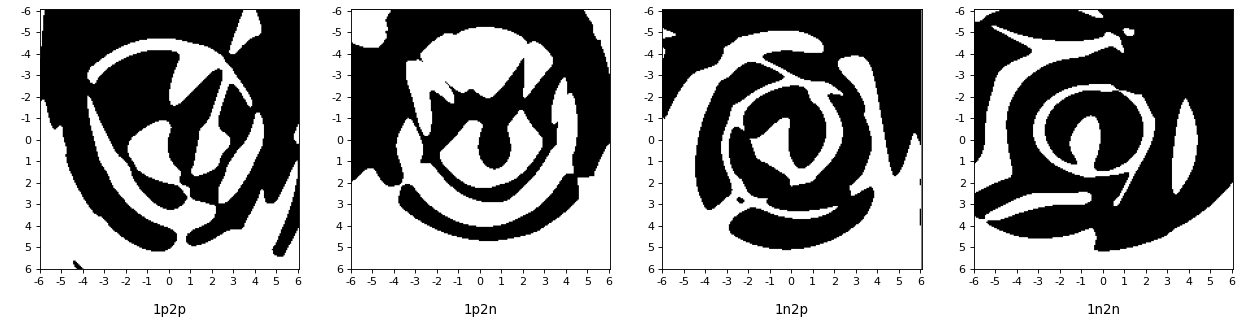
\includegraphics[width=1.0\textwidth]{figures/minmax_random_each_boundary.png}
        \caption{随机拆分min-max每个子模型的决策边界}
        \label{Fig-minmax-random-each-boundary}
    \end{figure}

    \begin{figure}[htbp]
        \centering
        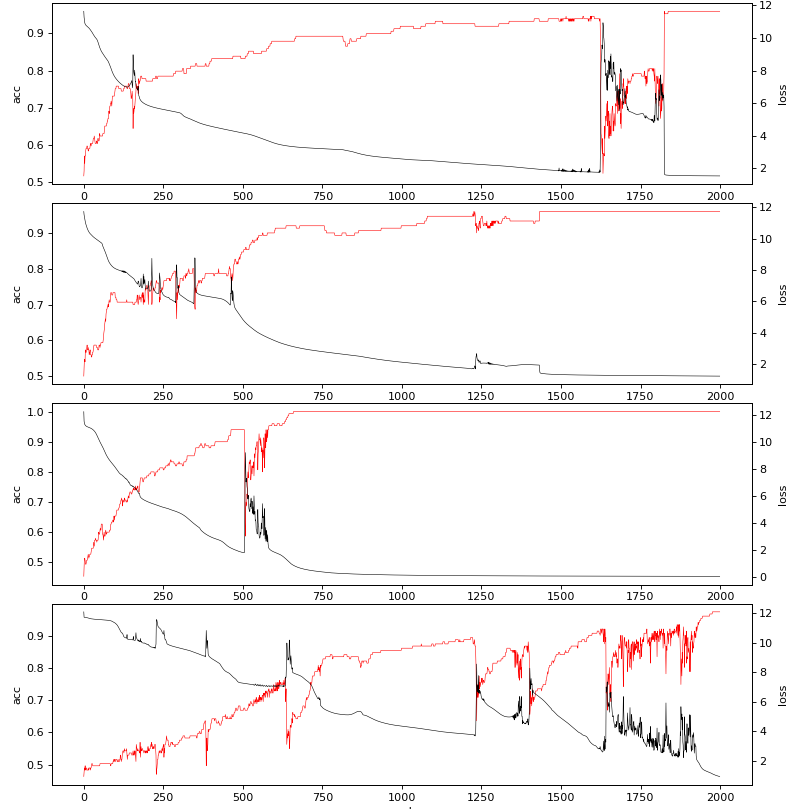
\includegraphics[width=1\textwidth]{figures/minmax_random_logging.png}
        \caption{随机拆分min-max每个子模型的损失函数、准确率变化}
        \label{Fig-minmax-random-logging}
    \end{figure}

\end{document}